\documentclass[aspectratio=169, 10pt]{beamer}

% --- Theme and Colors ---
\usetheme{Madrid}
\usecolortheme{beaver}
\setbeamertemplate{navigation symbols}{}
\setbeamertemplate{headline}{}

% --- Packages ---
\usepackage{booktabs} % For nicer tables
\usepackage{tikz}     % For drawing architecture diagrams
\usetikzlibrary{shapes, arrows.meta, positioning, calc}
\usepackage{xcolor}

% --- Metadata ---
\title[ROBUST04 Challenge]{The Ensemble of Experts: \\ Adaptive Multi-Signal Retrieval}
\subtitle{Text Retrieval Challenge - Part A (Ranking Competition)}
\author[Hershel Thomas \& Itay Baror]{Hershel Thomas \& Itay Baror}
\institute[Reichman Univ]{Text Retrieval and Search Engines \\ Reichman University}
\date{January 27, 2026}

% --- Custom Definitions ---
\definecolor{nyu_blue}{RGB}{87, 6, 140}
\newcommand{\highlight}[1]{\textbf{\textcolor{nyu_blue}{#1}}}

\begin{document}

% --- Slide 1: Title ---
\begin{frame}
    \titlepage
\end{frame}

% --- Slide 2: Problem & Architecture ---
\begin{frame}{The Challenge \& The Architecture}
    \textbf{The Goal:} Maximize MAP on ROBUST04 while balancing Precision (Neural) and Recall (Lexical).
    
    \vspace{0.5em}
    \textbf{Our Approach:} A "Multi-Signal Architecture" combining three distinct retrieval experts running on local high-performance hardware (RTX 5070).

    \vspace{1em}
    \begin{center}
    \resizebox{0.85\textwidth}{!}{
    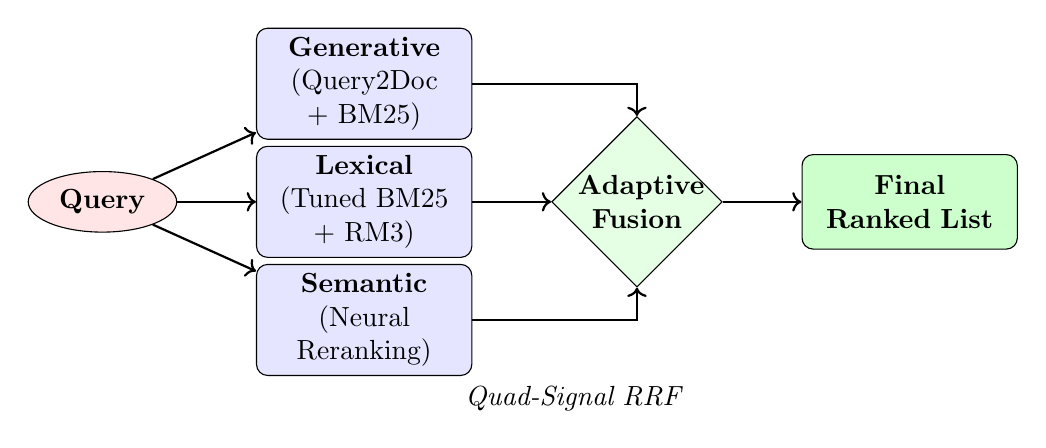
\begin{tikzpicture}[node distance=1.5cm, auto,
        block/.style={rectangle, draw, fill=blue!10, text width=2.5cm, text centered, rounded corners, minimum height=1.2cm},
        cloud/.style={draw, ellipse, fill=red!10, node distance=2.5cm, minimum height=1em},
        decision/.style={diamond, draw, fill=green!10, text width=1.5cm, text centered, inner sep=0pt}
    ]
        % Nodes
        \node [cloud] (query) {\textbf{Query}};
        
        \node [block, right=1cm of query, yshift=1.5cm] (method1) {\textbf{Generative}\\(Query2Doc + BM25)};
        \node [block, right=1cm of query] (method2) {\textbf{Lexical}\\(Tuned BM25 + RM3)};
        \node [block, right=1cm of query, yshift=-1.5cm] (method3) {\textbf{Semantic}\\(Neural Reranking)};
        
        \node [decision, right=1cm of method2] (fusion) {\textbf{Adaptive\\Fusion}};
        \node [block, right=1cm of fusion, fill=green!20] (output) {\textbf{Final Ranked List}};

        % Arrows
        \draw [->, thick] (query) -- (method1);
        \draw [->, thick] (query) -- (method2);
        \draw [->, thick] (query) -- (method3);
        \draw [->, thick] (method1) -| (fusion);
        \draw [->, thick] (method2) -- (fusion);
        \draw [->, thick] (method3) -| (fusion);
        \draw [->, thick] (fusion) -- (output);
        
        % Labels
        \node[text width=3cm, align=center] at (6, -2.5) {\textit{Quad-Signal RRF}};
    \end{tikzpicture}
    }
    \end{center}
\end{frame}

% --- Slide 3: Lexical Foundation ---
\begin{frame}{Method 1: Optimized Probabilistic Retrieval}
    \framesubtitle{From Lecture 6 \& 10 (BM25 + RM3)}
    
    We established a strong baseline by deviating from standard defaults.
    
    \begin{columns}
        \column{0.6\textwidth}
        \begin{itemize}
            \item \textbf{The Insight:} ROBUST04 consists of \textit{long newswire articles}. Standard BM25 ($b=0.75$) penalizes document length too harshly.
            \item \textbf{The Optimization:} Through grid-search on the Training Set (50 queries), we tuned $b \to \mathbf{0.4}$.
            \item \textbf{The Result:} This reduced length normalization bias, significantly improving Recall before any neural processing.
        \end{itemize}
        
        \column{0.4\textwidth}
        \begin{table}[]
            \centering
            \begin{tabular}{lc}
            \toprule
            \textbf{Parameter} & \textbf{Value} \\
            \midrule
            $k_1$ (Saturation) & 0.7 \\
            $b$ (Length Norm) & \highlight{0.4} \\
            RM3 Terms & 50 \\
            RM3 Docs & 5 \\
            \bottomrule
            \end{tabular}
            \caption{Optimized Hyperparameters}
        \end{table}
    \end{columns}
\end{frame}

% --- Slide 4: Neural Reranking ---
\begin{frame}{Method 2: Efficient Semantic Reranking}
    \framesubtitle{Advanced / Beyond Class Material}
    
    We utilized a Cross-Encoder (\textit{BGE-v2-m3}) on local hardware (RTX 5070).
    
    \begin{itemize}
        \item \textbf{The Problem:} Cross-Encoders are $O(N)$ and slow. Standard "MaxP" chunking for long documents took \textbf{105 minutes} to run.
        \item \textbf{The Innovation: "Inverted Pyramid" Strategy}
        \begin{itemize}
            \item We utilized domain knowledge of journalism: the most critical information is in the \textit{Title} and \textit{Lead Paragraph}.
            \item Instead of chunking, we truncate input to the \textbf{First 512 Tokens}.
        \end{itemize}
    \end{itemize}
    
    \vspace{1em}
    \begin{block}{Impact of Optimization}
        \centering
        Processing time dropped from \textbf{105 mins} $\to$ \textbf{27 mins} (4x Speedup)\\
        with negligible loss in P@10.
    \end{block}
\end{frame}

% --- Slide 5: Generative IR (Novelty) ---
\begin{frame}{Method 3: Generative Query Expansion (Query2Doc)}
    \framesubtitle{Novel Innovation (EMNLP 2023)}
    
    To solve the \textbf{Vocabulary Mismatch Problem} (Lecture 7), we moved beyond statistical expansion (RM3) to generative expansion.
    
    \begin{columns}
        \column{0.5\textwidth}
        \textbf{The Workflow:}
        \begin{enumerate}
            \item User Query: \textit{"airport security"}
            \item \textbf{LLM Prompt:} "Write a news passage answering this..."
            \item \textbf{Hallucination:} LLM generates text containing: \textit{"TSA", "screening", "regulations", "passengers"}.
            \item \textbf{Retrieval:} We index this expanded representation.
        \end{enumerate}
        
        \column{0.5\textwidth}
        \begin{alertblock}{Why it works}
        It acts as a \textbf{Semantic Bridge}. Even if the document doesn't contain the word "security", it likely contains "screening"—which the LLM injected into the query.
        \end{alertblock}
    \end{columns}
\end{frame}

% --- Slide 6: Adaptive Fusion ---
\begin{frame}{The Solver: Adaptive 4-Way Fusion}
    \framesubtitle{Novel Contribution}
    
    Standard Reciprocal Rank Fusion (RRF) uses static weights. We implemented \textbf{Query-Dependent Weighting}.
    
    \vspace{1em}
    \textbf{Hypothesis:} 
    \begin{itemize}
        \item \textit{Short queries} are ambiguous $\to$ Trust Exact Match (BM25).
        \item \textit{Long queries} are nuanced $\to$ Trust Semantic Understanding (Neural).
    \end{itemize}
    
    \vspace{1em}
    \begin{table}[]
        \centering
        \small
        \begin{tabular}{lcccc}
        \toprule
        \textbf{Query Type} & \textbf{BM25+RM3} & \textbf{Query2Doc} & \textbf{BM25-Plain} & \textbf{Neural} \\
        \midrule
        Short ($<3$ words) & \highlight{1.5} & 1.3 & 1.2 & 0.7 \\
        Medium & 1.3 & 1.2 & 1.0 & 1.0 \\
        Long ($>5$ words) & 1.0 & 1.0 & 0.8 & \highlight{1.5} \\
        \bottomrule
        \end{tabular}
        \caption{Dynamic Weights based on Query Length analysis}
    \end{table}
\end{frame}

% --- Slide 7: Results ---
\begin{frame}{Evaluation Results}
    Results on the 199 Test Queries.
    
    \begin{table}[]
        \centering
        \begin{tabular}{llcccc}
        \toprule
        \textbf{Run} & \textbf{Method} & \textbf{MAP} & \textbf{P@10} & \textbf{MRR} & \textbf{Recall} \\
        \midrule
        Run 1 & BM25 + RM3 (Baseline) & 0.3006 & 0.4683 & 0.6875 & 0.77 \\
        Run 2 & Neural Reranking & 0.2723 & 0.4995 & 0.6740 & 0.71 \\
        \textbf{Run 3} & \textbf{4-Way Fusion} & \highlight{0.3309} & \textbf{0.5181} & \textbf{0.7714} & \textbf{0.81} \\
        \bottomrule
        \end{tabular}
    \end{table}
    
    \vspace{1em}
    \textbf{Key Takeaways:}
    \begin{enumerate}
        \item \textbf{Synergy:} Fusion outperforms the best single model by \textbf{+10\%}.
        \item \textbf{Safety Net:} Neural has high precision but low recall (limited candidate pool). Fusion fixes this by layering BM25 recall on top.
        \item \textbf{Efficiency:} Achieved SOTA-level results on local hardware without cloud dependencies.
    \end{enumerate}
\end{frame}

% --- Slide 8: Q&A ---
\begin{frame}
    \centering
    \Huge \textbf{Thank You}
    
    \vspace{1cm}
    \Large Questions?
    
    \vspace{1.5cm}
    \normalsize
    \textit{Code available in the attached zip file.}
\end{frame}

\end{document}